\documentclass[10pt]{article}
\usepackage[a4paper,margin=1.25cm,top=1.0cm,bottom=1.0cm]{geometry}
\usepackage{amsmath,amssymb,graphicx,booktabs,microtype,xcolor}
\usepackage[font=footnotesize,labelfont=bf,skip=3pt]{caption}
\usepackage{enumitem,float}
\setlist{nosep,leftmargin=1.2em}
\setlength{\parindent}{0pt}\setlength{\parskip}{1.5pt}
\usepackage{titlesec}
\titlespacing*{\section}{0pt}{5pt}{2pt}
\titleformat{\section}{\normalsize\bfseries}{\thesection}{0.6em}{}
\titleformat{\subsection}[runin]{\small\bfseries}{}{0em}{}[.]
\titlespacing*{\subsection}{0pt}{3pt}{0.5em}
\newcommand{\amin}{^{\prime}}
\pagestyle{empty}
\begin{document}

{\large\bfseries Close pairs and blending of SZ clusters on a Poisson halo sky}\\[1pt]
{\small Analytic results checked against full-sky simulations \hfill code \& full report: \texttt{sz-poisson-blending/} \quad 10 November 2026}

\section{Set-up}
\begin{itemize}
\item \textbf{Halos.} Tinker08 HMF ($M_{500c}$), Planck18, $10^{13}<M_{500}/M_\odot<10^{16}$, $0.01<z<3$. Positions: a Poisson process on the full sky (no clustering).
\item \textbf{Signal.} Planck 2013 $Y_{500}$--$M_{500}$, $(1-b)=0.8$, $\sigma_{\ln Y}=0.173$; Arnaud GNFW profile cut at $5R_{500}$.
\item \textbf{Instrument.} Beam FWHM $1.4\amin$; white noise $4\times10^{-6}$ (y-arcmin); no CMB or foregrounds.
\item \textbf{Detection.} Matched filter at the cluster's own $\theta_{500}$. $q=Y_{500}/\sigma_Y(\theta_{500})$, $q_{\rm obs}=q+\mathcal N(0,1)$, cut at $q_{\rm cut}=4$--$7$.
\item \textbf{Counts.} $2.93\times10^7$ halos above $10^{13}$, $3.96\times10^5$ above $10^{14}$. Detections at $q_{\rm cut}=4,5,6,7$: $132\,125$, $85\,912$, $61\,630$, $46\,575$, i.e.\ $\Sigma_{\rm det}=3.20,\,2.08,\,1.49,\,1.13~{\rm deg^{-2}}$.
\end{itemize}

\section{Analytic results}
\subsection{Q1: $N$ clusters in an aperture}
Selecting by mass, $q_{\rm obs}$ or $z$ thins a Poisson process, and the result is still Poisson. For surface density $\Sigma$ and a cap of radius $\theta$:
\begin{equation*}
\mu=\Sigma\,2\pi(1-\cos\theta)\simeq\Sigma\pi\theta^2,\qquad P(N=n)=e^{-\mu}\mu^n/n!,\qquad P(\ge k)=1-\textstyle\sum_{j<k}e^{-\mu}\mu^j/j!\;.
\end{equation*}
\begin{itemize}
\item \textbf{Centred on a detected cluster.} The \emph{other} objects follow the same ${\rm Pois}(\mu)$ (Slivnyak--Mecke). This also holds for neighbours from another population $B$, with $\mu_B=\Sigma_BA(\theta)$, whatever the centre's $z$ or $q$. Do not count the centre.
\item \textbf{$k$-th neighbour.} $P(d_k\le\theta)=\gamma(k,\mu)/\Gamma(k)$.
\item \textbf{Whole sky.}
  \begin{itemize}
  \item Pairs closer than $\theta$: $E=\bar N\mu/2$, ${\rm Var}=E(1+2\mu)$.
  \item Triples with all separations $<\theta$: $\bar N\mu^2p_3/6$, $p_3=1-3\sqrt3/4\pi$.
  \item Chance that at least one such configuration exists: $1-e^{-E}$.
  \end{itemize}
\item \textbf{Flat sky.} $\pi\theta^2$ is off by a factor $\simeq1+\theta^2/12$, which only matters above about $5^\circ$.
\end{itemize}

\subsection{Q2: blending at a threshold}
Neighbour $B$ adds $x_B=\rho(\theta_A,\theta_B,s_{AB})\,Y_B/\sigma_Y(\theta_A)$ to the SNR of primary $A$. Here $\rho$ is the filter's cross-response, with $\rho=1$ for a source at the centre. The blended SNR is $q_b=q_A+n+\delta-\mu_{\bar y}$, with $\delta=\sum_Bx_B$. Four outcomes are counted:
\begin{itemize}
\item \textbf{B1, merged pair:} two detectable clusters within $\theta_b$. $\;f_{\rm B1}=1-e^{-\Sigma_{\rm det}A(\theta_b)}$.
\item \textbf{B2, contamination:} $Y$ over-estimated by more than $\varepsilon$.
\item \textbf{B3, boosting:} detected only thanks to neighbours.
\item \textbf{Lost:} detectable alone but not detected, either absorbed into a brighter peak or pushed below threshold.
\end{itemize}
The summed neighbour signal is \emph{compound Poisson} (the ``P(D)'' of confusion theory):
\begin{equation*}
\phi_\delta(k)=\exp\!\Big[\int\!dx\,R(x)\,\big(e^{ikx}-1-ikx\big)\Big],\qquad
R(x)=\!\int\! dz\,d\ln M\,d\ln Y\,\frac{d^3N}{d\Omega\,dz\,d\ln M}\,p(\ln Y)\!\int\! d^2s\;\delta_D\!\big(x-\rho Y/\sigma_A\big).
\end{equation*}
The $-ikx$ term removes the map mean. By Slivnyak's theorem the same law holds around a halo as around a random point. Fractions are taken \emph{over the selected sample}, and $A$ must be the brightest contributor:
\begin{equation*}
f_{\rm B2}=\frac{\int dN_A\,e^{-\Lambda(x>q_A)}\!\int d\delta\,p(\delta)\,\mathbf 1[\delta-\mu_{\bar y}>\varepsilon q_A]\,\Phi(q_A+\delta-\mu_{\bar y}-q_{\rm cut})}{\int dN_A\,e^{-\Lambda(x>q_A)}\!\int d\delta\,p(\delta)\,\Phi(q_A+\delta-\mu_{\bar y}-q_{\rm cut})}\,,
\end{equation*}
where $\Lambda(x>q_A)=\int_{q_A}^\infty R(x)\,dx$ is the expected number of neighbours brighter than $A$. B3 and Lost follow from the same integrand.
\begin{itemize}
\item \textbf{The filter sees the mean $y$.} A white-noise matched filter is not compensated, so it responds to the mean $\bar y$ through $\mu_{\bar y}=\bar y\,\sigma_A\,{\rm RATIO}/N_w$, where ${\rm RATIO}$ is the filter's response to a uniform $y$ background and $N_w$ the white-noise level. With $\bar y=6.4\times10^{-7}$ this is a shift of $0.4\sigma$ ($0.5\amin$ filter) to $3\sigma$ ($10\amin$). Without mean removal, blending fractions roughly triple and do not converge as the mass floor is lowered.
\item \textbf{Selection.} A detection is more likely to pass the cut when its neighbours add signal. So formulas that ignore selection, such as $1-e^{-\lambda}$, underestimate contamination by $\times1.3$--$1.5$.
\end{itemize}

\section{Simulations}
\begin{itemize}
\item \textbf{Q1.} 120 full-sky catalogues, plus $2\times1000$ skies with a mass floor and $20\,000$ skies of rare objects. Neighbours counted with KD-trees on the sphere for $0.5\amin$--$60\amin$ and $N=0$--$6$.
\item \textbf{Q2, catalogue level.} The P(D) compared with direct sums over 60 skies.
\item \textbf{Q2, map level.} $324$ flat patches of $10^\circ\times10^\circ$ ($32\,400\,{\rm deg^2}$). Every halo above $10^{13}M_\odot$ painted, noise added, map mean removed. Then a 12-scale matched filter ($0.5\amin$--$10\amin$), peaks taken at the maximum SNR over scales and merged within $2\amin$. Each peak is split exactly into per-halo contributions.
\item \textbf{Checks.} Every number was confirmed by two independent re-implementations or re-run on fresh seeds.
\end{itemize}

\begin{figure}[H]
\centering
\begin{minipage}[c]{0.44\textwidth}
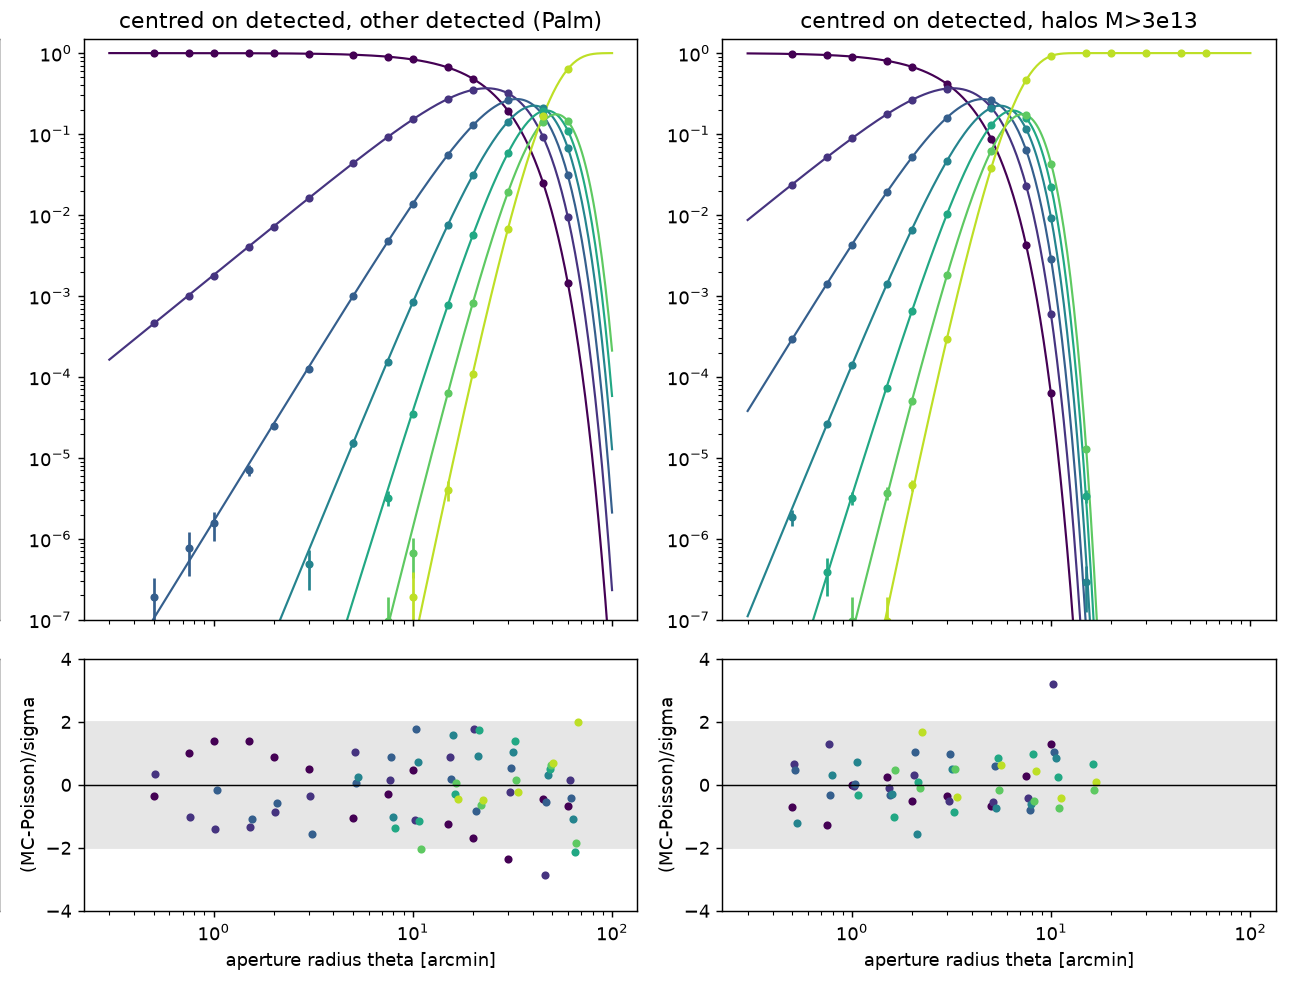
\includegraphics[width=\linewidth]{f1.png}
\end{minipage}\hfill
\begin{minipage}[c]{0.54\textwidth}
\captionof{figure}{$P(N=n)$ of \emph{other} objects within $\theta$ of a detected ($q>5$) cluster, over 120 full skies. Left: other detections. Right: halos with $M>3\times10^{13}$. Lines are ${\rm Pois}(\mu)$ with no free parameter; colours run from $n=0$ (dark) to $n\ge6$ (yellow). Bottom panels: residuals in $\sigma$. A sky bootstrap gives a global $p=0.40$.}
\vspace{4pt}
\footnotesize
\begin{tabular}{@{}l cccc@{}}
\toprule
$P(\ge1$ neighbour$)$, $q>5$ centre & $1\amin$ & $2\amin$ & $5\amin$ & $10\amin$\\
\midrule
other detection ($q>5$) & 0.18\% & 0.72\% & 4.4\% & 16.6\%\\
halo $M>10^{14}$ & 0.84\% & 3.3\% & 18.9\% & 56.8\%\\
halo $M>3\times10^{13}$ & 9.3\% & 32\% & 91\% & 99.99\%\\
$P(\ge2)$, other detections & $2\!\times\!10^{-6}$ & $3\!\times\!10^{-5}$ & 0.10\% & 1.5\%\\
\midrule
pairs on the full sky & 78 & 312 & 1952 & 7807\\
\bottomrule
\end{tabular}\\[2pt]
{\scriptsize Monte Carlo agrees to rms $0.8\sigma$ over 72 entries. MC triples at $5\amin$: $17.2\pm0.4$ (analytic 17.3).}
\end{minipage}
\end{figure}

\begin{figure}[H]
\centering
\begin{minipage}[c]{0.28\textwidth}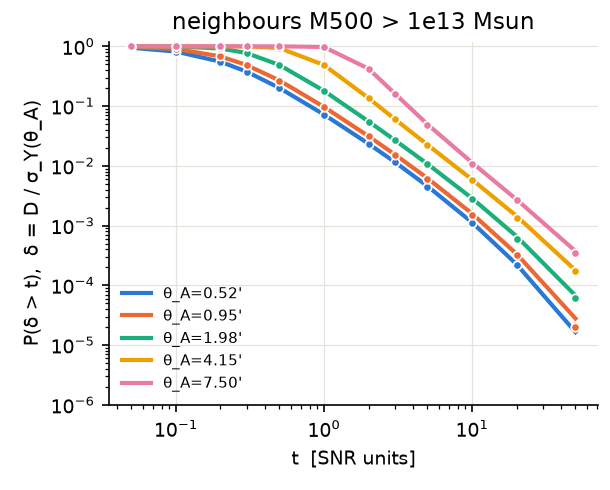
\includegraphics[width=\linewidth]{f2a.png}\end{minipage}\hfill
\begin{minipage}[c]{0.31\textwidth}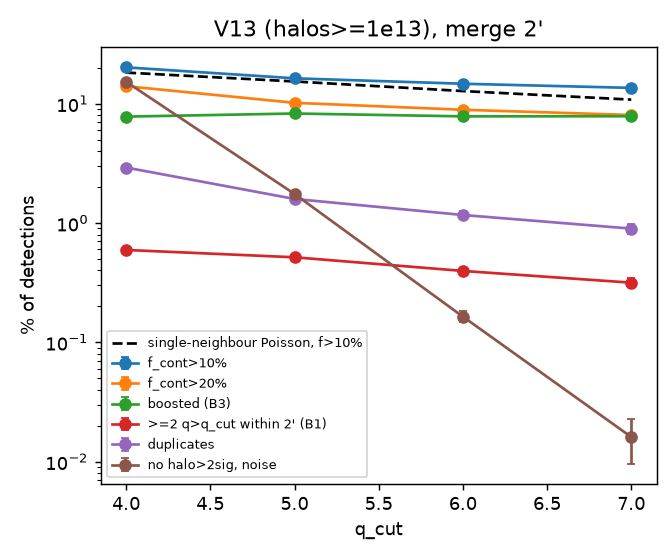
\includegraphics[width=\linewidth]{f2b.png}\end{minipage}\hfill
\begin{minipage}[c]{0.385\textwidth}
\captionof{figure}{\textbf{Left:} probability that the summed neighbour signal in a filter of scale $\theta_A$ exceeds $t$ (in units of the noise $\sigma$). Lines: compound-Poisson FFT. Points: direct sums over 60 skies (rms $z=0.93$ in the tail). \textbf{Right:} map-level blending versus $q_{\rm cut}$, as a fraction of \emph{all} map peaks. Projected neighbours (blue, orange, green) dominate. Merged pairs of detectable clusters (red) stay below 0.6\%. Pure-noise peaks (brown) matter only at $q_{\rm cut}=4$.}
\end{minipage}
\end{figure}

\begin{table}[H]
\centering\footnotesize
\caption{Blending versus $q_{\rm cut}$. Cat.: analytic compound-Poisson fractions of blended detections; Monte Carlo agrees to rms $z=0.98$ over 363 tests. Map: fractions of real map detections (the denominator excludes noise peaks, unlike Fig.~2), $\pm0.1$--$0.2\%$. Lost: percentage of halos detectable alone that are not detected.}
\begin{tabular}{@{}c c cc cc cc cc@{}}
\toprule
& B1 (map) & \multicolumn{2}{c}{B2: $Y$ bias $>10\%$} & \multicolumn{2}{c}{B2: $Y$ bias $>20\%$} & \multicolumn{2}{c}{B3: boosted} & \multicolumn{2}{c}{Lost}\\
$q_{\rm cut}$ & $\ge2$ det.\ in $2\amin$ & cat. & map & cat. & map & cat. & map & cat. & map\\
\midrule
4 & 0.59\% & 18.5\% & 13.7\% & 12.4\% & 7.8\% & 8.7\% & 7.8\% & 10.9\% & 11.8\%\\
5 & 0.52\% & 16.2\% & 14.5\% & 10.5\% & 8.4\% & 8.1\% & 8.3\% & 9.0\% & 9.7\%\\
6 & 0.40\% & 14.5\% & 13.8\% & 9.1\% & 8.1\% & 7.6\% & 7.8\% & 7.9\% & 8.5\%\\
7 & 0.32\% & 13.1\% & 12.9\% & 8.1\% & 7.4\% & 7.1\% & 7.5--7.9\% & 7.1\% & 7.5\%\\
\bottomrule
\end{tabular}
\end{table}

\section{Robustness and beyond Poisson}
\begin{itemize}
\item \textbf{Instrument and model.} Across 11 noise, beam, $z_{\max}$ and HMF variants, Q1 stays Poisson ($\chi^2=124/124$); only $\Sigma_{\rm det}$ changes. Contamination and boosting scale by $\times1.3$ for noise $\times0.5$, $\times1.4$ for a $5\amin$ beam, and $\times0.95$ for a different HMF. Y-scatter has no effect.
\item \textbf{Mass floor.} With the mean removed, a floor of $10^{13}$ is converged. Halos above $10^{14}$ supply $\sim$83\% of B2 and B3.
\item \textbf{Clustering} (Limber, Tinker10 bias) multiplies close-pair probabilities by $1+\bar w=1.13$--$1.27$ at $1$--$5\amin$ and blending fractions by $\times1.08$--$1.13$.
\item \textbf{Halo exclusion} is negligible: about $0.1\%$ of detected close pairs overlap in 3D. Blending is projection along the line of sight.
\item \textbf{The detected catalogue is not Poisson.} Neighbours boost each other over the threshold, so close pairs at $2$--$5\amin$ are $1.5$--$2.7\times$ the Poisson rate. Pairs closer than about $0.35\,$FWHM are suppressed.
\end{itemize}

\section{Conclusions}
\begin{itemize}
\item \textbf{Q1 is purely geometric.} $P(N)={\rm Pois}(\Sigma A)$ for random or cluster-centred apertures and for any selection. Simulations confirm it to $\lesssim1\sigma$. For an SO-like survey at $q>5$, 0.7\% of clusters have another detection within $2\amin$, while a third have a $>3\times10^{13}$ halo there.
\item \textbf{Q2 is dominated by confusion, not by pairs.} Merged pairs of detectable clusters are only about 0.5\% of detections. About 15\% of $q>5$ detections have $Y$ biased by more than 10\% by mostly undetectable halos at other redshifts. About 8\% exist only because of that boost, and about 10\% of detectable halos are lost.
\item \textbf{No single blending radius describes contamination.} The radius needed to reproduce B2 grows from $8\amin$ to $12\amin$ with $q_{\rm cut}$. Use the compound-Poisson P(D) with the map mean removed and selection applied. It matches the map ground truth to within $\sim$2 percentage points.
\item \textbf{Recipe.} (i) Compute $\Sigma_{\rm det}(q_{\rm cut})$ from HMF $\times$ completeness. (ii) Q1: ${\rm Pois}(\Sigma A)$, multiplied by $1+\bar w$ if clustering matters. (iii) Q2: build $R(x)$ from the filter cross-response with halos down to $\sim10^{13}$, FFT to P(D), convolve with the noise, apply the cut and the brightest-contributor rule. (iv) Calibrate absorption against your own peak finder by injecting into maps.
\end{itemize}
\end{document}
